\section{Модель Изинга на прямоугольной решётке}

В данном разделе мы будем рассматривать зависимость наблюдаемых модели Изинга от формы решетки: в частности, от отношения сторон в прямоугольной решётке

\subsection{Расчёт критических кумулянтов для модели прямоугольного Изинга}

Кумулянт Биндера для модели Изинга в критической точке расчитывается по формуле:
\begin{equation}
\label{eq:Cumulant}
U_{4} = 1 - \frac{\la m^{4} \ra}{3 (m^{2})^{2}}
\end{equation}

где $\la m^{2} \ra$ - средний квадрат удельной намагниченности, $\la m^{4} \ra$ - средная удельная намагниченность в четвертой степени. 

Для сравнения значения кумулянтов модели прямоугольного Изинга с разными размерами, но одинаковым отношением сторон (так же Aspect Ratio или r), так, что число спинов составляет $L \times rL$ были проведены симуляции модели на основе алгоритма из проектной работы Сорокина Никиты \cite{web:SchroedingercatRepos} и Камиллы Файзулиной \cite{web:SAWsRepos} - для этого были взяты длины L = 50, 100, 200 и 400 и отношения сторон r = 1/4, 1/2, 3/4 при $2 * 10^{6}$ итераций. Все расчёты проводились в критической точке\cite{selke2006critical}:

\begin{equation}
\label{eq:Crit_Dot}
J = \frac{1}{2.26918...}
\end{equation}



\begin{figure}[!h]
    \centering
    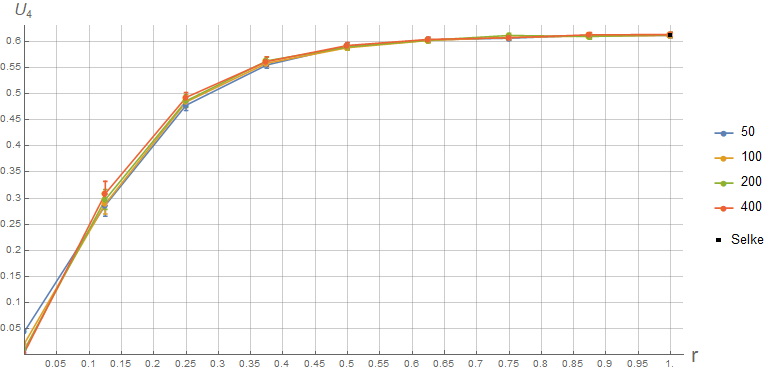
\includegraphics[width=110mm]{Sections/Images/CumulantPBC.png}
    \vfill
    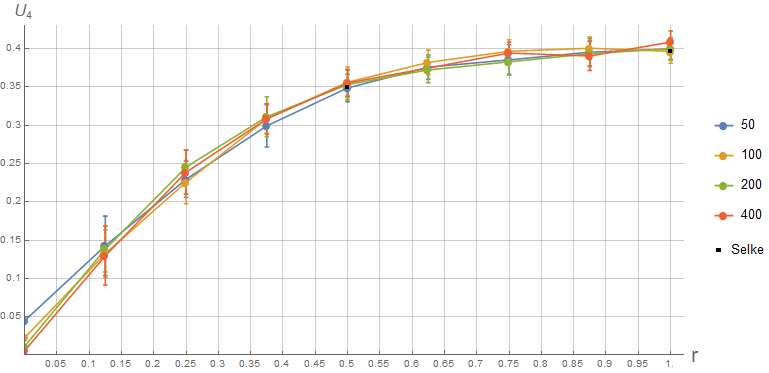
\includegraphics[width=110mm]{Sections/Images/CumulantOBC.png}
    \caption{График зависимости значения кумулянта Биндера \eqref{eq:Cumulant} в крит. точке \eqref{eq:Crit_Dot} от Aspect Ratio при открытых (снизу) и периодических гран. условиях (сверху). Черные точки - значения критических кумулянтов из работы W. Selke\cite{selke2006critical}}
    \label{fig:CumulOPBC}
\end{figure}

Крайние левые точки в отметке нуля являются расчётами для модели одномерного Изинга (где длина цепочки равна соответствующей стороне в двумерном изинге). Так, в случае открытых гран. условий (рис. \ref{fig:CumulOPBC} cнизу) и периодических (рис. \ref{fig:CumulOPBC} сверху) значения кумулянта стремится к нулю с увеличением длины цепочки(см. Проект6.pdf\cite{web:ProjectMagnetRepos}).
Черными точками отмечены значения критического кумулянта из работы Уолтера Сельке\cite{selke2006critical}:

\begin{table}[]
    \centering
    \begin{tabular}{|c|c|c|}
        \hline
        Boundary & r & $U_{4}$ \\ \hline
        OBC & 1 & $0.396 \pm 0.002$ \\ \hline
        OBC & 0.5 & $0.349 \pm 0.002$\\ \hline
        PBC & 1 & 0.61069...\\ \hline
    \end{tabular}
    \caption{Таблица значений критических кумулянтов для прямоугольных решёток из статьи У. Сельке \cite{selke2006critical}}
    \label{tab:U4_Selke}
\end{table}

Эти же значения отмечены в графиках \ref{fig:CumulOBCL} и \ref{fig:CumulPBCL} зависимости крит. кумулянта от обратной длины стороны как крайние левые (в нуле - так обозначен случай термодинамического предела).

\begin{figure}[!h]
    \centering
    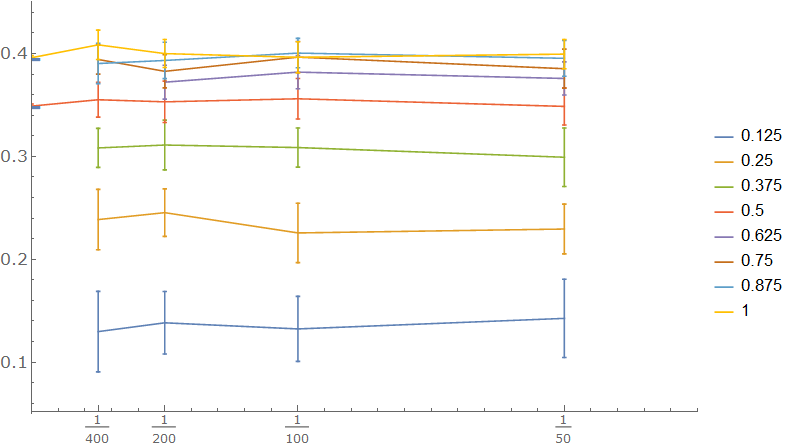
\includegraphics[width=100mm]{Sections/Images/CumulantOBCL.png}
    \caption{График зависимости значения кумулянта Биндера в крит. точке от обратной длины стороны при открытых гран. условиях}
    \label{fig:CumulOBCL}
\end{figure}

\begin{figure}[!h]
    \centering
    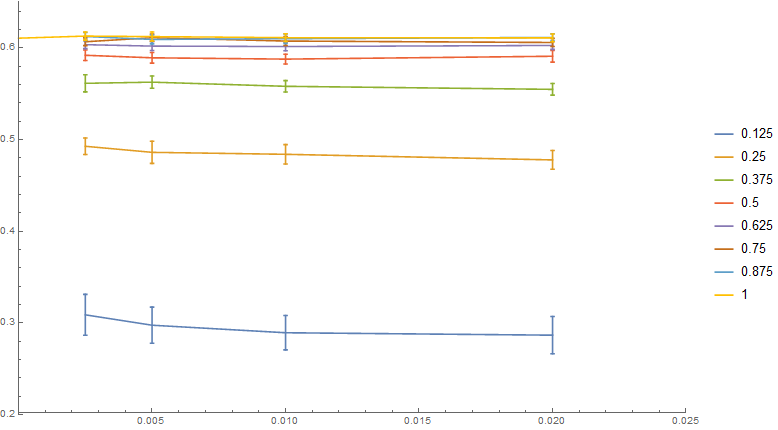
\includegraphics[width=100mm]{Sections/Images/CumulantPBCL.png}
    \caption{График зависимости значения кумулянта Биндера в крит. точке от обратной длины стороны при периодических гран. условиях}
    \label{fig:CumulPBCL}
\end{figure}

Учитывая погрешность в расчётах симуляций, зависимость от обратной длины прямоугольника 1/L не наблюдается.

\subsection{Сравнение модели Изинга и модели взаимодействующих непересекающихся блужданий}

Здесь мы рассмотрим основные понятия в модели взаимодействующих блужданий (Self-Avoiding Walks, SAWs), связанные с их формой и сравним их с прямоугольной моделью в тех же условиях. 

Важнейшим параметром в описании полученной симуляциями Монте-Карло блуждания из N узлов является радиус инерции, численно равный среднему квадратическому расстоянию частиц (i-я частица в блуждании имеет вектор $w_{i}$) от положения среднего арифметического центра система (сумма $w_{k}$ в скобке)\cite{caracciolo2011geometrical}:

\begin{equation}\label{eq:Rg}
    R^{2}_{g} = \frac{1}{N+1} \sum^{N}_{i=0}\left(w_{i} - \frac{1}{N+1}\sum^{N}_{k=0}w_{k}\right)^2 = \frac{1}{2(N+1)^{2}}\sum^{N}_{i,j=0}(w_{i} - w_{j})^{2}
\end{equation}

(Под операцией возведения вектора или разности векторов в квадрат подразумевается сумма квадратов элементов вектора) Так же для описания формы модели применяется тензор вращения относительно центра масс - матрица, $\alpha\beta-$й элемент которой расчитывается по формуле (4) из статьи\cite{arkin2013gyration} :

\begin{equation}\label{eq:Ten_G1}
    Q_{N,\alpha\beta} = \frac{1}{N+1} \sum^{N}_{i=0}(w_{i,\alpha} - w_{c, \alpha})(w_{i,\beta} - w_{c, \beta})
\end{equation}
где $w_{c,\alpha} - \alpha$ -я координата вектора центра масс. В случае, если начало координат расположено в центре масс (следовательно, сумма векторов точек блуждания = 0), формула $\alpha\beta-$элемента тензора упрощается и численно равна второму моменту координаты (если $\alpha = \beta$), или до среднего произведения разных координат по всем точкам блуждания.


\begin{align}\label{eq:Ten_G_C}
    Q_{N,\alpha\beta} = &\frac{1}{(N+1)} \sum_{i=0}^{N} w_{i, \alpha} w_{i, \beta} \\
    \sum^{N}_{i=0}w_{i} &= 0
\end{align}

Рассмотрим формулу \eqref{eq:Ten_G1}. Так так $w{c}$ - центра масс блуждания, то:

\begin{equation}
    w_{c} = \frac{1}{N+1} \sum_{k=0}^{N} w_{k}
\end{equation}

Так же можно представить i-й вектор блуждания как:

\begin{equation}
    w_{i} = \frac{1}{N+1} \sum_{k=0}^{N} w_{i}
\end{equation}

Это позволит нам вытащить из скобок N+1 и избавиться от неизвестного $w_{c}$

\begin{align*}
    Q_{N,\alpha\beta} = \frac{1}{(N+1)^{3}} \sum^{N}_{i=0}(\sum^{N}_{k=0}(w_{i,\alpha} - w_{k, \alpha}))(\sum^{N}_{l=0}(w_{i,\beta} - w_{l, \beta})) = \\
    = \frac{1}{(N+1)^{3}} \sum^{N}_{i=0} \sum^{N}_{k,l=0}(w_{i,\alpha} - w_{k, \alpha})(w_{i,\beta} - w_{l, \beta}) = \\
    \frac{1}{(N+1)^{3}} \sum^{N}_{i=0} \sum^{N}_{k,l=0} (w_{i,\alpha} w_{i,\beta} - w_{i,\alpha} w_{l,\beta} - w_{k,\alpha} w_{i,\beta} + w_{k,\alpha} w_{l,\beta})
\end{align*}

Расскроем суммирование у учётов зависимостей индексов:

\begin{align*}
    Q_{N,\alpha\beta} = \frac{1}{(N+1)^{2}} (\sum^{N}_{i,k=0}(w_{i,\alpha} w_{i,\beta}) - \sum^{N}_{i,l=0}(w_{i,\alpha} w_{l,\beta}) - \sum^{N}_{i,k=0}(w_{k,\alpha} w_{i,\beta}) + \sum^{N}_{k,l=0}(w_{k,\alpha} w_{l,\beta})) = \\
    \frac{1}{(N+1)^{2}} \sum^{N}_{i,k=0}(w_{i,\alpha} w_{i,\beta} - w_{k,\alpha} w_{i,\beta}) = \frac{1}{2(N+1)^{2}} \sum^{N}_{i,k=0}(w_{i,\alpha} - w_{k, \alpha})(w_{i,\beta} - w_{k, \beta})
\end{align*}
т.к. кол-во произведений координат разных векторов и одинаковых меньше в два раза. Полученная формула:

\begin{equation}\label{eq:Ten_G2}
    Q_{N,\alpha\beta} = \frac{1}{2(N+1)^{2}} \sum^{N}_{i,k=0}(w_{i,\alpha} - w_{k, \alpha})(w_{i,\beta} - w_{k, \beta})
\end{equation}

совпадает с формулой (4.1) из статьи о взаимодействующих блужданиях\cite{caracciolo2011geometrical}, что значит что используемое ими понятие "тензора вращения" совпадает.

\subsection{Связь тензора инерции и тензора вращения}

Можно заметить некоторое сходство в расчётах недиагональных элементов тензора инерции J и тензора вращения из статей\cite{caracciolo2011geometrical,arkin2013gyration}. Действительно, для системы из N материальных точек единичной массы тензор инерции в системе центра масс рассчитывается следующим образом:

\begin{equation}
\label{eq:Ten_I_J}
    J = \left(
    \begin{array}{ccc}
        J_{xx} & J_{xy} & J_{xz}  \\
        J_{yx} & J_{yy} & J_{yz} \\
        J_{zx} & J_{zy} & J_{zz}
    \end{array} \right)
\end{equation}

\begin{align}
    J_{xy} &= J_{yx} = -\sum_{i=1}^{N} x_{i} y_{i} \\
    J_{yz} &= J_{zy} = -\sum_{i=1}^{N} y_{i} z_{i} \\
    J_{xz} &= J_{zx} = -\sum_{i=1}^{N} x_{i} z_{i} 
\end{align}

В тоже время, формулы диагональных элементов принципиально отличаются:

\begin{align}
    J_{xx} &= \sum_{i=1}^{N} y_{i}^{2} + z_{i}^{2} \\
    J_{yy} &= \sum_{i=1}^{N} x_{i}^{2} + z_{i}^{2} \\
    J_{zz} &= \sum_{i=1}^{N} x_{i}^{2} + y_{i}^{2}
\end{align}

Сравнивая с формулой элементов тензора вращения в системе центра масс \eqref{eq:Ten_G_C}, можно заметить, что недиагональные элементы тензоров отличаются знаком и усреднением в тензоре вращения. Диагональные же элементы "противоположны" друг другу:
в тензоре инерции они обозначают осевые моменты инерции (относительно $O_{\alpha}$, и поэтому обозначенные моменты одной координатой ($J_{\alpha\alpha}$ используют сумму квадратов отличных от $\alpha$ координат.

Таким образом, элементы тензора вращения в системе центра масс в трехмерном пространстве можно представить как:

\begin{equation}
   Q_{\alpha\alpha} = \frac{1}{N}\sum^{N}_{i=1}w_{i,\alpha}^2 = \frac{1}{N} \left(\sum_{i=1}^{N}x_{i}^{2} + y_{i}^{2} + z_{i}^{2} - J_{\alpha\alpha}\right) = R^{2}_{g} - \frac{1}{N} J_{\alpha\alpha}  
\end{equation}

где $w_{i,\alpha}$ - $\alpha$-я координата радиус-вектора i-й материальной точки.

\begin{equation}
    Q_{\alpha\beta} = -\frac{1}{N} J_{\alpha\beta},\ \ \alpha \neq \beta
\end{equation}

Тогда матричный вид формулы тензора вращения \eqref{eq:Ten_G_C} через тензор инерции \eqref{eq:Ten_I_J} будет:

\begin{equation}
    Q = R_{g}^{2} * E - \frac{1}{N} J
\end{equation}
где E - это единичная матрица порядка, совпадающим с размерностью данной модели Dim.

Мы знаем, что симметричная матрица (какой являются и Q, и J) всегда диагонализируема, а базис из собственных векторов - ортогонален. Пусть S - матрица перехода в жорданов базис тензора инерции. Произведём переход в этот базис для тензора вращения:

\begin{equation*}
    S^{T}QS = S^{T} (R_{g}^{2} * E - \frac{1}{N} J) S = R^{2}_{g} * S^{T}ES-\frac{1}{N} * S^{T}JS
\end{equation*}

Матрица S - ортогональна, следовательно $S^{-1} = S^{T}$, поэтому:

\begin{equation}
    S^{T}QS = R^{2}_{g} * E - \frac{1}{N} * J_{D}
\end{equation}

где $J_{D}$ - диагонализированная матрица тензора инерции. Очевидно, что полученная в правой части матрица - диагональная. Следовательно, матрица в левой части так же получилась диагональной полсе перехода в новый базис и жорданов базис тензоров инерции и вращения одинаковы, пусть и с разными собственными значениями. Соответствующие собственные значения матриц в жордановом базисе будут равны:

\begin{align*}
    (S^{T}QS)_{ii} = Q_{D, ii} = R^{2}_{g} - \frac{1}{N}J_{ii},\ \ i=1..Dim
\end{align*}

Стоит подчеркнуть, что если жорданов базис составлен так, что собственные значения тензора инерции в матрице упорядочены по неубыванию, то в тензоре вращения собственные значения в матрице в этом базисе же будут упорядочены по невозрастанию.

\subsection{Показатели формы блуждания из тензора вращения}

Так как полученная матрица симметричная, то существует такой поворот, преобразующий её в диагональную (т.е., приводящий систему в Жорданов базис с собственными значениями по диагонали, и нулевыми недиагональными элементами), причём так, чтобы значения на диагонали были положительными и упорядоченными по невозрастанию.

В нашем двумерном случае, 

\begin{equation*}
    Q_{N} = \left(
    \begin{array}{cc}
      q_{1} & 0 \\
      0 & q_{2}
    \end{array} \right),\ 0 < q_{2} \leq q_{1}
\end{equation*}

Отметим так же, что сумма диагональных элементов тензора вращения равна квадрату радиуса вращения и инвариантна. Определим ещё один показатель формы из статьи Пелиссетто\cite{caracciolo2011geometrical}:

\begin{align*}
    s_{1} &= \frac{\la q_{1} \ra_{N}}{\la R_{g}^{2} \ra_{N}}\\
    s_{2} &= 1 - s_{1} = \frac{\la q_{2} \ra_{N}}{\la R_{g}^{2} \ra_{N}}\\
    r_{12} &= \frac{s_{1}}{1-s_{1}}
\end{align*}

Учитывая, что в $s_{1}$ и $s_{2}$ значения в числителе и знаменателе являются квадратами средних квадратичных значений, то следует вывод, что $\sqrt{r_{12}}$ является знакомым нам отношением сторон из предыдущего подраздела, только в данном случае это отношение не сторон прямоугольника, а полуосей эллипса инерции, который образует полученая симуляциями модель-блуждание.

Так же из статьи Пелиссетто\cite{caracciolo2011geometrical} определим среднюю асферичность (показатель, насколько блуждание отличается от круга):

\begin{equation}
\label{eq:Asphericity}
    \mathcal{A} = \La \frac{(q_{1} - q_{2})^{2}}{(q_{1} + q_{2})^{2}} \Ra_{N}
\end{equation}

\subsection{Асферичность прямоугольных решёток}

Асферичность необходима в следующем подразделе для оценки формы как блужданий в моделях взаимодействующих непересекающихся блужданий ISAW и Изинга на полимерной цепочке, так и прямоугольных решёток для модели Изинга: существует явная зависимость между отношением сторон r (точнее, отношением числа спинов по горизонтали (L) и по вертикали (r x L)) и значением асферичности соответствующей решётки:

\begin{figure}[h]
\begin{minipage}{0.45\textwidth}
     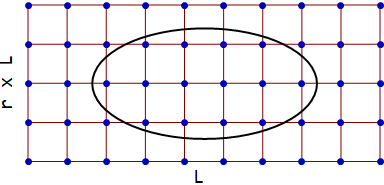
\includegraphics[width=\textwidth]{Sections/Images/RectanGrid.png}
    \caption{Пример прямоугольной решётки со стороной L = 10 и отношением сторон r = 0.5 и её эллипс инерции, полуоси которого рассчитаны по формулам \eqref{eq:i_x} и \eqref{eq:i_y}}
\end{minipage}
\hfill
\begin{minipage}{0.5\textwidth}
     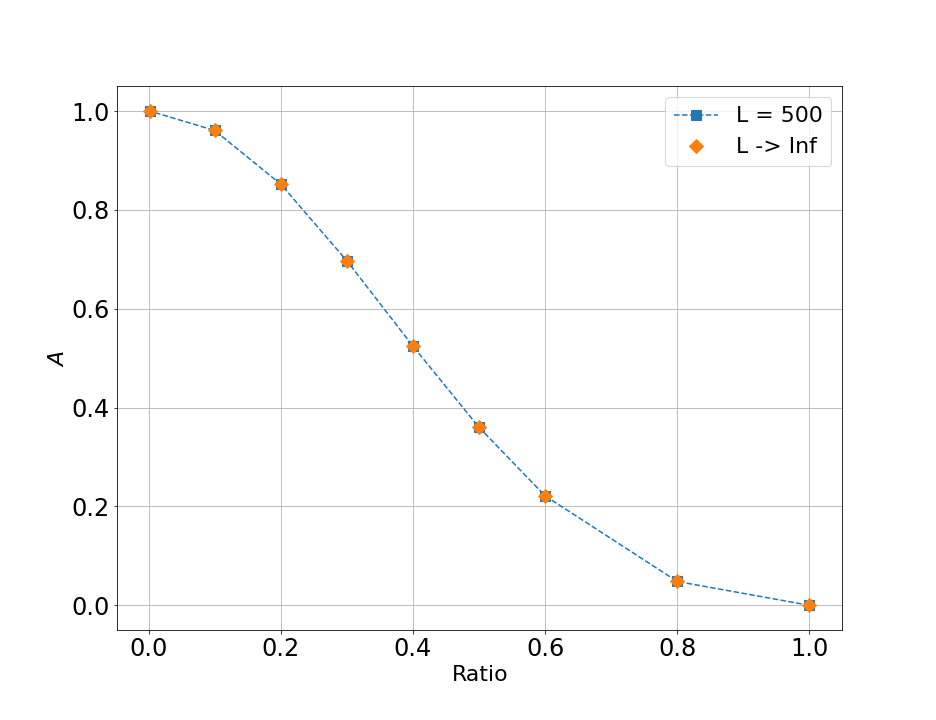
\includegraphics[width=\textwidth]{Sections/Images/A_r.png}
    \caption{График зависимости значения асферичности прямоугольной решётки длины 500 и в случае бесконечно большой длины от отношения сторон Ratio (или r)}
    \label{fig:A_r}
\end{minipage}
   
\end{figure}

\begin{table}[h!]
    \begin{minipage}{0.45\textwidth}
    \centering
    \begin{tabular}{|c|c|c|} 
    \hline
        L & r & $\mathcal{A}$ \\ \hline
        10 & \multirow{3}{*}{0.5}  &  0.371802 \\ \hhline{-~-}
        100 & & 0.360115 \\ \hhline{-~-}
        1000 &  & 0.360001 \\ \hline
        \multirow{9}{*}{500} & 1.0 & 0 \\ \hhline{~--}
        & 0.8 & 0.048186 \\\hhline{~--}
        & 0.6 & 0.221455 \\\hhline{~--}
        &0.5 & 0.360004 \\\hhline{~--}
        &0.4 & 0.524383 \\\hhline{~--}
        &0.3 & 0.697005 \\\hhline{~--}
        &0.2 & 0.852084 \\\hhline{~--}
        &0.1 & 0.960803 \\\hhline{~--}
        &0.002 (1D) & 1 \\\hline
    \end{tabular}
    \caption{Таблица зависимости значения асферичности прямоугольной решётки от стороны L и отношения сторон r. Значения для длины 500 соответствуют значениям из графика \ref{fig:A_r}}
    \label{tab:A_L_r}    
    \end{minipage}
    \hfill
    \begin{minipage}{0.45\textwidth}
    \centering
    \begin{tabular}{|c|c|c|} 
    \hline
        r & $\mathcal{A}$ \\ \hline
        1.0 & 0 \\ \hline
        0.8 & 0.0481856 \\\hline
        0.6 & 0.221453 \\\hline
        0.5 & 0.36 \\\hline
        0.4 & 0.524374 \\\hline
        0.3 & 0.696995 \\\hline
        0.2 & 0.852071 \\\hline
        0.1 & 0.960788 \\\hline
        0(1D) & 1 \\\hline
    \end{tabular}
    \caption{Таблица зависимости значения асферичности прямоугольной решётки бесконечно большой длины стороны L от отношения сторон r, отмеченная оранжевыми точками в графике \ref{fig:A_r} и рассчитанные по формуле \eqref{eq:AsperScaled}}
    \label{tab:A_L_r}    
    \end{minipage}
\end{table}

Центр эллипса инерции совпадает с центром прямоугольной решётки, полуоси лежал вдоль сторон и их длины равны:

\begin{align}
    i_{x} = \sqrt{\frac{J_{xx}}{N}} \label{eq:i_x}\\
    i_{y} = \sqrt{\frac{J_{yy}}{N}}
    \label{eq:i_y}
\end{align}

Здесь необходимо подчеркнуть, что моменты инерции считаются относительно осей в базисе, в которой тензор инерции обращается в диагональную матрицу. При этом нужно отметить, что $i_{x}$ - длина полуоси, перпендикулярной оси oX, и наоборот, $i_{y}$ - длина полуоси, перпендикулярной оси oY того же базиса. Поэтому для упрощения следующих расчётов мы сразу будет считать, что центр прямоугольника лежит в начале координат, а стороны параллельны осям координат - при таких условиях недиагональные элементы тензора инерции обращаются в ноль. 

Рассмотрим зависимость получаемой асферичности прямоугольной решётки с нефиксированными отношением сторон r и стороной L, чтобы оценить шкалирование данной величины от L, заметное из таблицы \ref{tab:A_L_r}. Для начала рассчитаем собственные значения тензора вращения.

\begin{figure}
    \centering
    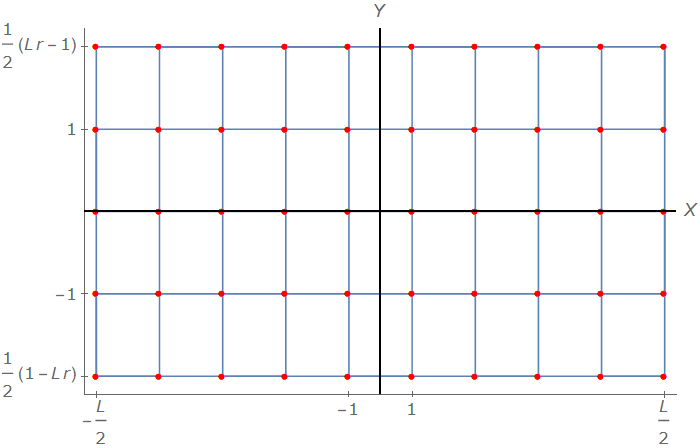
\includegraphics[width=100mm]{Sections/Images/RectanGrid2.png}
    \caption{Модель прямоугольной решётки для расчётов асферичности - она имеет четную и нечетную стороны, чтобы можно было рассмотреть всевозможные случаи}
    \label{fig:Rectan2}
\end{figure}

В случае, когда сторона прямоугольной решётки четна (то есть, имеет чётное количество узлов), решётка будет иметь по $L/2$ спинов слева и справа от начала координат. Причем координаты узлов решётки будут иметь $L/2$ различных по модулю значений абсциссы, повторяющихся $rL$ раз. Тогда из \eqref{eq:Ten_G_C}, где $N = L \times (r \times L)$:
\begin{align*}
q_{xx} &= \frac{(r\times L) \sum^{L/2}_{i=1}2(i-0.5)^{2}}{(r\times L) L} = \frac{\sum^{L/2}_{i=1}(2i^{2}-2i-0.5)}{L} = \\
&=\frac{0.5 L/2}{L} - 2\frac{1+2+...+L/2}{L} + 2\frac{1 + 4 + ... + L^{2}/4}{L} = \\
&=\frac{1}{4} - \frac{2}{L} \frac{L/2(L/2+1)}{2} + \frac{2}{L} \frac{L/2(L/2+1)(L+1)}{6} = \\
&=\frac{1}{4} - \frac{L}{4} - \frac{1}{2} + \frac{L^{2}}{12} +\frac{3L}{12} + \frac{1}{6} = \frac{L^{2}-1}{12}
\end{align*}

Если же сторона прямоугольника нечётна, то один ряд будет лежать на оси и не будет участвовать в расчётах q для соответствующей оси (в случае из рисунка \ref{fig:Rectan2} - $q_{yy}$ из \eqref{eq:Ten_G_C}):

\begin{align*}
    q_{yy} &= \frac{2 L\sum_{i=1}^{(rL-1)/2}i^{2}}{(r \times L) \times L} = \frac{2}{r L} (1 + 4 + ... + (r L -1)^{2}/4) = \\
    &= \frac{2}{r L} \frac{(r L-1)/2 \times (r L+1)/2 \times r L}{6} = \frac{(r L)^{2} - 1}{12}
\end{align*}

Из этого следует, что чётность сторон не влияет на собственные значения тензора вращения и для прямоугольников они равны:
\begin{align}
    q_{xx} &= \frac{L^{2}-1}{12} \label{eq:Qx} \\
    q_{yy} &= \frac{(r L)^{2} - 1}{12}
    \label{eq:Qy}
\end{align}

\

Перейдём непосредственно к расчёту асферичности по определению \eqref{eq:Asphericity}: 
\begin{align*}
    \mathcal{A} &= \frac{(q_{1} - q_{2})^{2}}{(q_{1} + q_{2})^{2}},\ q_{1} \geqslant q_{2} \Rightarrow \left[ q_{1} = q_{xx},\ q_{2} = q_{yy} \right] \\
    \mathcal{A} &= \left(\frac{L^{2} - (rL)^{2}}{L^{2} + (rL)^{2} - 1/6}\right)^{2} = \left( \frac{1 - r^{2}}{1 + r^{2} - 1/(6L^{2})} \right)^{2} = \left( \frac{1-r^{2}}{1+r^{2}} +  \right)^{2} = \\
    &= \left( \frac{1-r^{2}}{1+r^{2}} + \frac{1-r^{2}}{6L^{2}(1-r^{2})^{2}} + O[\frac{1}{L^{4}}] \right)^{2} = \\
    &= \left( \frac{1-r^{2}}{1+r^{2}}\right)^{2} + \left( \frac{1-r^{2}}{6L^{2}(1+r^{2})^{2}} \right)^{2} + \frac{1-r^{2}}{3L^{2}(1+r^{2})^{3}} + O[\frac{1}{L^{4}}] = \\
    &= \left( \frac{1-r^{2}}{1+r^{2}}\right)^{2} + O[\frac{1}{L^{2}}]
\end{align*}

В итоге, получаем:

\begin{equation}
    \mathcal{A} = \left( \frac{1-r^{2}}{1+r^{2}}\right)^{2} + O[\frac{1}{L^{2}}]
    \label{eq:AsperScaled}
\end{equation}



\subsection{Свойства моделей вблизи фазового перехода с учётом показателей формы}

Цель данного раздела - сравнить кумулянты Биндера в области фазового перехода у трёх моделей - гомополимер (далее взаимодействующее блуждание или ISAW), модель Изинга на полимерной цепочке (далее PolIsing) и модель Изинга на прямоугольной решётке (далее "прямоугольный Изинг"). В отличие от первых двух моделей, отношение сторон прямоугольного Изинга является параметром модели, а не наблюдаемой величной. Следовательно, цель - сравнить крит. кумулянты моделей с прямоугольным Изингом, имеющим те же показатели формы, что имеют ISAW и PolIsing в области фазового перехода. 
Для этого для первых двух моделей была рассчитана зависимость значения асферичности A \eqref{eq:Asphericity} от константы взаимодействия J при длиннах N = 1000, 2500, 3600, 4900.
\newpage
\begin{figure}[h!]
    \centering
    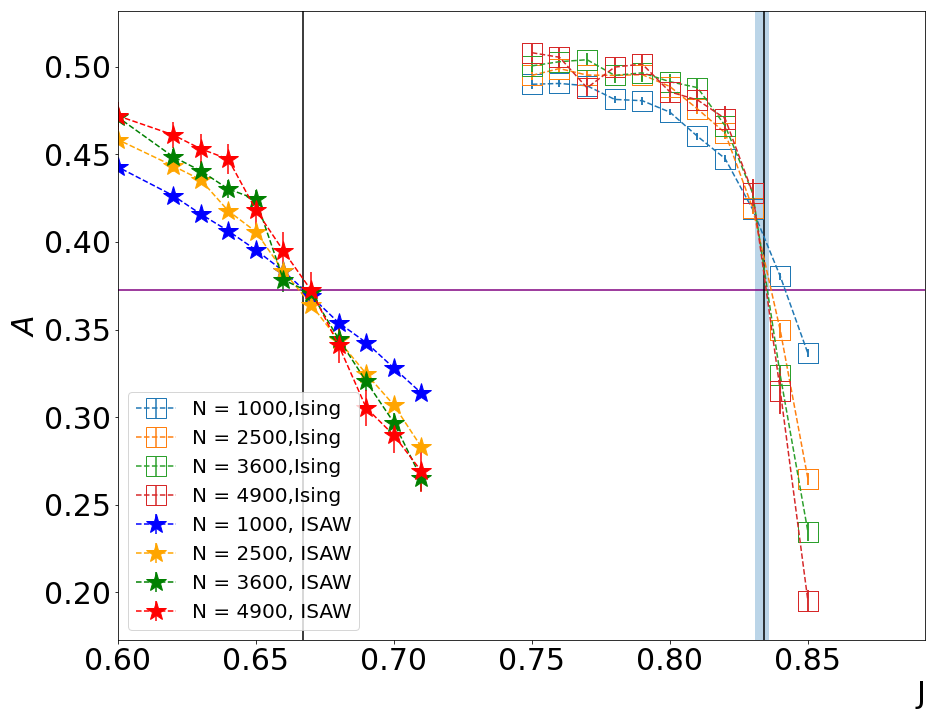
\includegraphics[width=150mm]{Sections/Images/Ising_ISAW_A_J_Full.png}
    \caption{График зависимости значения асферичности от константы взаимодействия для моделей взаимодействующего блуждания (слева) и Изинга на полимерной цепочке (справа)}
    \label{fig:A_J}
\end{figure}

Вертикальными линиями обозначены точки фазового перехода моделей: красными линиями отмечены граничные с точки зрения погрешности точки перехода в модели Изинга на гомополимерной цепочке ($0.833 \pm 0.003$, или $T_{c}=1/J_{c} = 1.199\pm0.003$\cite{foster2021critical}), а черной сплошной - у модели ISAW($\approx 0.667$\cite{caracciolo2011geometrical}). Горизонтальной линией отмечено значение асферичности в критической области модели ISAW из статьи Пелиссетто, равное 0.3726(7) ((4.10)\cite{caracciolo2011geometrical}). Однако перед тем как найти значение кумулянта для модели прямоугольного Изинга, необходимо подобрать такое отношение сторон, чтобы асферичность полученного прямоугольника совпадала со значением асферичности в точках перехода соответствующих моделей.

\begin{figure}[h!]
\begin{minipage}{0.45\textwidth}
    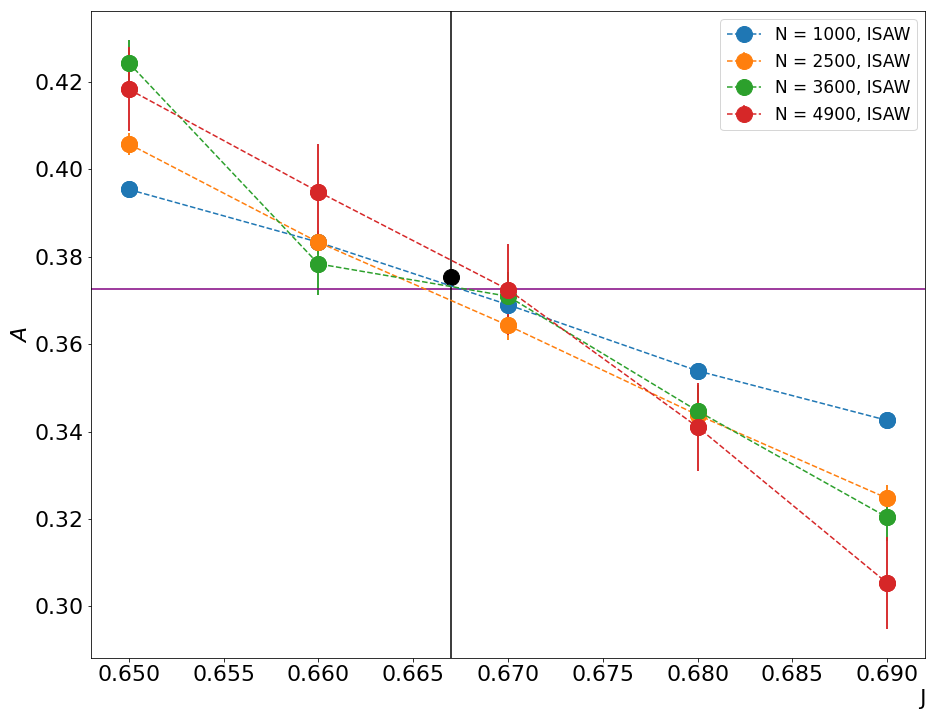
\includegraphics[width=\textwidth]{Sections/Images/ISAW_A_J_Close.png}
    \caption{График \ref{fig:A_J}, увеличенный в масштабе в области фазового перехода модели взаимодействующих блужданий}
    \label{fig:ISAW_A_J_Zoom}
\end{minipage}
\hfill
\begin{minipage}{0.45\textwidth}
    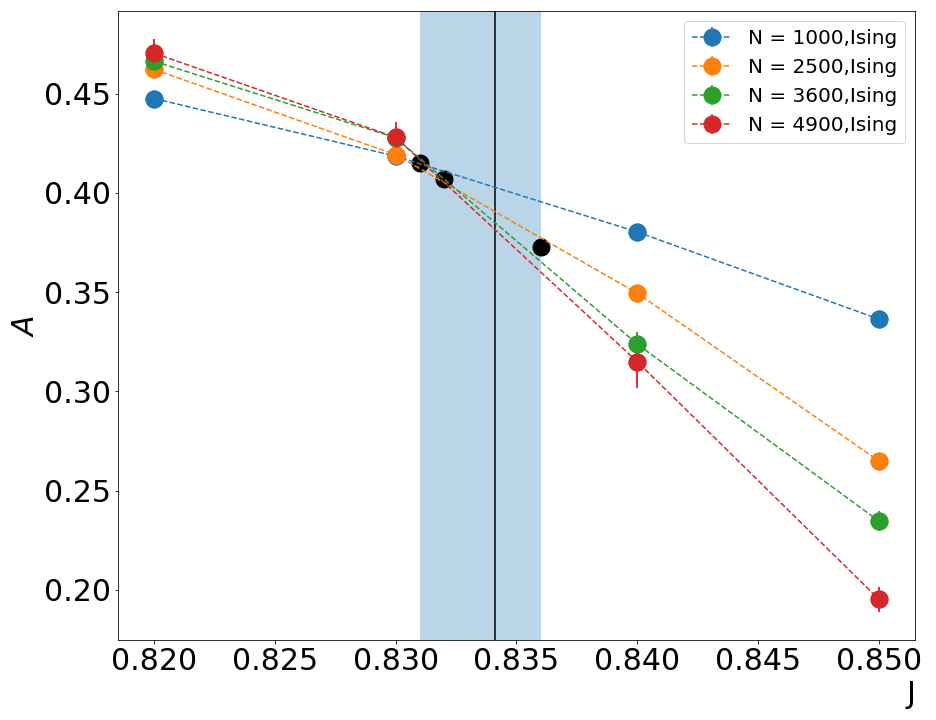
\includegraphics[width=\textwidth]{Sections/Images/Ising_A_J_Close.png}
    \caption{График \ref{fig:A_J}, увеличенный в масштабе в области фазового перехода Изинга на полимерной цепочке. }
    \label{fig:Is_A_J_Zoom}
\end{minipage}

\end{figure}

\newpage

Чёрные точки на графиках \ref{fig:ISAW_A_J_Zoom}-\ref{fig:Is_A_J_Zoom} будут точками, для которых мы будет подбирать отношение сторон для модели прямоугольного Изинга по значению асферичности. Для модели PolIsing точки в красных линиях показывают среднее значение асферичности в граничных точках перехода - по ним мы определим погрешность измерений кумулянта: $r = 0.465$ и $0.49$, $U_{4} = 0.340\pm0.006$ и $0.348\pm0.006$. В точке на зелёной линии - в точке ближайшей к пересечению (переходу) рассчитаем само значение кумулянта: $r = 0.47,\ U_{4} = 0.343\pm0.006$. Тогда значение критического кумулянта модели Изинга в прямоугольной решётке для PolIsing $U_{4} = 0.343\pm0.009$

Для ISAW критический кумулянт прямоугольного Изинга рассчитан для $r=0.49$ и равен $0.349 \pm 0.006$ соответственно.

\begin{table}[h!]
    \centering
    \begin{tabular}{|c|c|c|c|}
        \hline
         \multicolumn{4}{|c|}{PolIsing}  \\ \hline
         J & $\mathcal{A}$ & r & $U_{4}\  Rectangular$ \\ \hline
         0.831 & 0.415 & 0.465 & $0.340 \pm 0.006$\\ \hline
         0.832 & 0.4072 & 0.47 & $0.343 \pm 0.006$\\ \hline
         0.836 & 0.373 & $0.490 \pm 0.002$ & $0.348 \pm 0.006$\\ \hline
         \multicolumn{4}{|c|}{ISAW} \\ \hline
         0.667 & 0.375 & 0.49 & $0.349 \pm 0.006$ \\ \hline
    \end{tabular}
    \caption{Таблица значений критических кумулянтов прямоугольной решётки в зависимости от асферичности моделей PolIsing и ISAW в областях крит. перехода и, следовательно, отношения сторон}
    \label{tab:my_label}
\end{table}

Сравнение со значением критического кумулянта модели PolIsing ($U_{4} = 0.308(8)$\cite{faizullina2021critical}), рассчитанное в статье Файзуллиной Камиллы, показало значительное несовпадение со значениями кумулянта прямоугольной решётки с теми же показателями формы, что и у рассматриваемой модели. 